Se caracterizan por transportar energía en forma de calor y pueden ser emitidos por cualquier objeto con una temperatura superior al cero absoluto, es decir 0 Kelvin (-273.15ºC). Se utilizan en medicina, electrónica, calefacción, astronomía y sistemas de seguridad.

\begin{figure}[H]
  \centering
  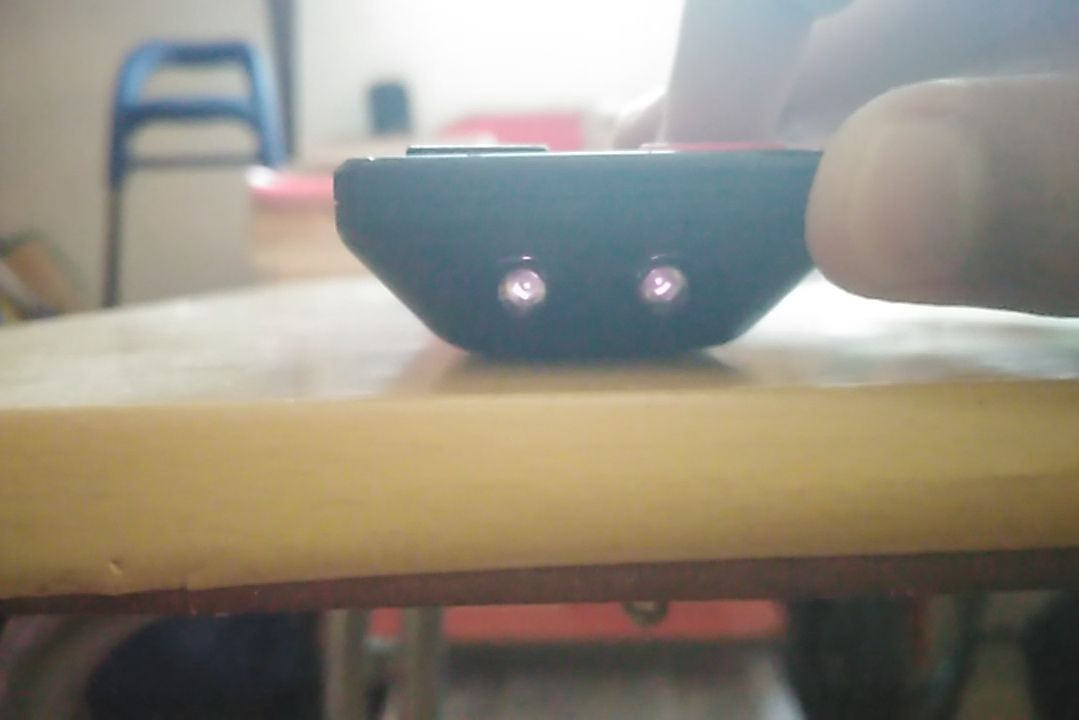
\includegraphics[scale=0.2]{imagenes/control_remoto.png}
  \caption{Rayos infrarrojos emitidos por un control remoto de televisor}
\end{figure}
